\chapter{Introduction}
\label{ch:introduction}
\section{Motivation}
% Heterogeneous Networks motivation..
There has been an exponential growth in the Internet landscape. The devices like smartphones, computers, laptops, tablets will continue to increase along with multitude of other devices that are connected to Internet. This has facilitated the research in dynamic spectrum access (DSA)~\cite{arhtn2,arhtn3} for efficient utilization of spectrum resources to sustain billions of Internet of Things (IoT) devices. There has been a significant increase in the study of cognitive radios for efficiently utilizing the electromagnetic spectrum. It has been observed that the spectrum occupancy is not uniform across all frequency bands, resulting in numerous spectral white spaces~\cite{bookhtn1}. To opportunistically access the idle channel, spectrum sensing is considered to be a significant technology enabling DSA. Although several spectrum sensing techniques have been proposed in the open literature, energy detection is widely used due to its low implementation complexity~\cite{arhtn4}. We discuss some of the spectrum sensing techniques along with energy detection below.
\begin{itemize}
\item In energy detection (ED) scheme the energy of the signal is detected in the frequency location and based on the threshold value we decide whether the signal is present or absent.

\item Cyclostationary Feature Detection is a complex scheme to implement compared to ED and it is mostly used when we need to also classify the signal present based on their modulation scheme.

\item When secondary user has a priori knowledge of primary user signal, matched  filter (MF)  detection  is  applied. Detection by using matched filter needs less detection time compared to ED but primary user information is required.
\end{itemize}

These spectrum sensing techniques can be used in a non-cooperative manner but it is very challenging to get an accurate estimate using a single-sensor system under a practical fading environment. Various non-idealities such as shadowing, multipath and fluctuating noise variance can make it difficult to detect the primary user~\cite{inphtn5,inphtn6}. Cooperative spectrum sensing can mitigate the effects of multipath and shadowing by utilizing the spatial and temporal diversity of a multiple radio network~\cite{inphtn7,inphtn8}. In cooperative spectrum sensing, each sensor node collects the spectral data and transmits it to a fusion center (FC) for decision making. Figure~\ref{fig:css} shows how a heterogeneous sensor network exploits the spatial diversity. 

\begin{figure}[!ht]
\label{fig:css}
\centering
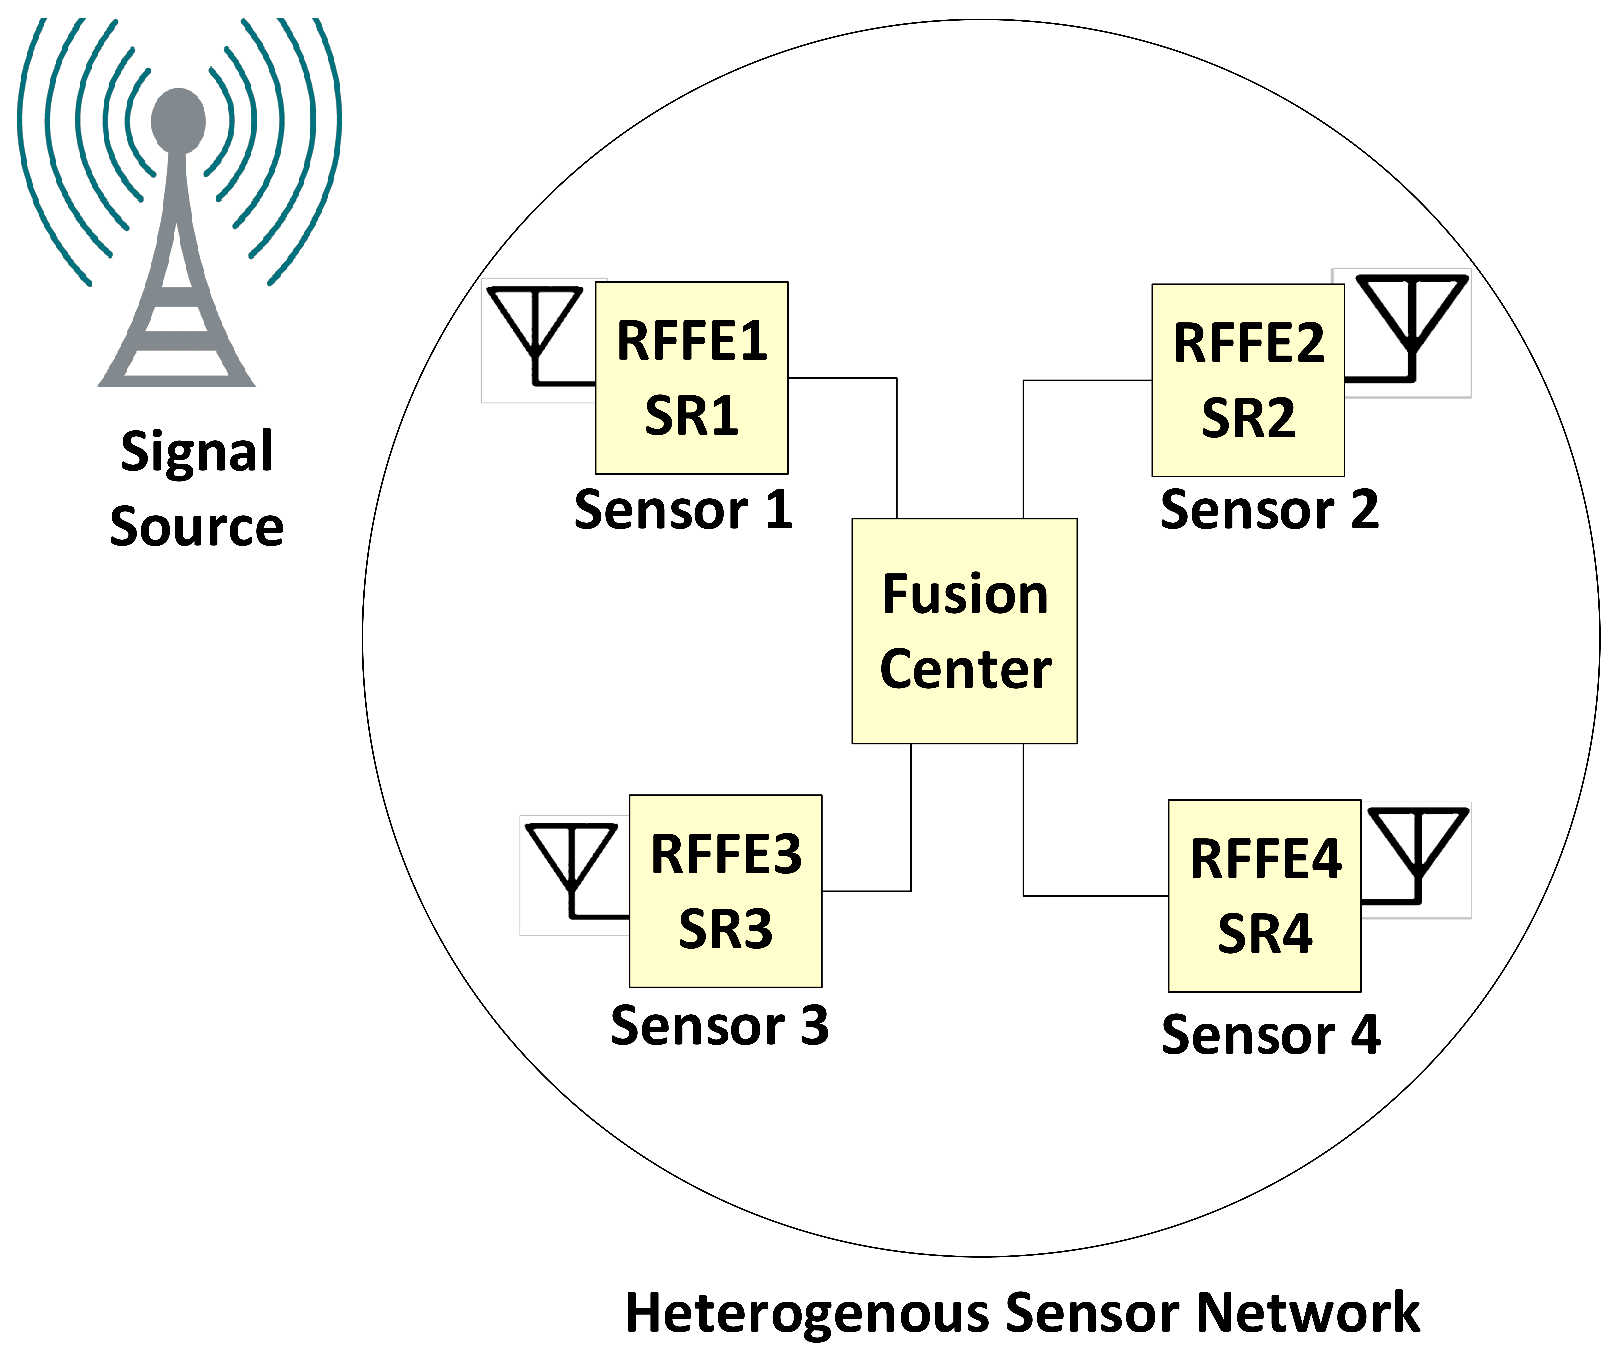
\includegraphics[width=0.75\textwidth,keepaspectratio]{images/Gill/figs/introdiag.eps} 
\caption{Heterogeneous sensor network employing cooperative spectrum sensing. $RFFE_i$ and $SR_i$ represents different front end and sampling rates for the SDR units.}
\end{figure}

% LTE-R Network motivation..
We have also analyze the performance of Long Term Evolution for Railways (LTE-R) in a tunnel environment. In recent years, the use of trains have witnessed tremendous growth due to their increasing speeds, which has led to the demand for reliable wireless communication systems with these transportation systems. The development of a reliable wireless network for high speed trains is not a simple task and it is still an emerging technology. Global System for Mobile Communication (GSM-R)~\cite{trlter1}, was a wireless communications standard designed for high speed trains, but it turned out not to be reliable enough and possess several limitations. Subsequently, LTE~\cite{trlter2} proposed a promising solution for achieving broadband data rates in high speed trains that can overcome various GSM-R limitations~\cite{arlter3,inplter4}. 

LTE-R is a high speed communication standard based on the existing LTE system architecture~\cite{inplter4}. There has been several studies regarding the assessment of LTE-R as a viable choice for next generation high speed communications for railway applications~\cite{inplter5,inplter6}. Most LTE systems operate at 1.8 GHz -- 2.6 GHz bands, which possesses a high propagation loss and severe fading effects. Highly mobile trains inside tunnel environment makes the design of reliable communication links very challenging. To achieve reliable radio coverage inside tunnels, leaky feeder cables have been proposed~\cite{arlter7}. With LCX, more uniform coverage can be achieved and installation is also comparatively simple. Each slot in the cable is equivalent to an antenna, which can transmit and receive signals. Figure~\ref{fig:ltertunnel} shows the LOS propagation environment inside a tunnel for a high speed train with velocity $v$.

\begin{figure}[!ht]
\label{fig:ltertunnel}
\centering
\includegraphics[width=0.75\textwidth,keepaspectratio]{images/Gill/lte_figs/3dtunnel.eps} 
\caption{High speed train inside a tunnel for LTE-R. $D_{LOS}$ is the distance between transmitter and receiver, $d$ is the distance between the LCX cable transmission slots.}
\end{figure}

\section{State of the Art}
% Heterogeneous Networks state-of-the-art..
The cooperative spectrum sensing testbed using normalized energy detection has been implemented and and has been compared for both soft and hard data fusion scheme. Both soft data fusion and hard data fusion have been extensively studied~\cite{arhtn9,inphtn10,arhtn11}, with several algorithms being implemented for each scheme. In a hard decision approach, each local decision statistic from sensor node is transmitted to an FC via overhead channels. The FC merges the sensing data and makes a global decision based on various algorithms such as majority rule, OR rule and AND rule~\cite{inhtn12}. For a soft decision scheme, each SU sends its local sensing data to the FC, which makes decision based on a global test statistic $G$. Soft decision combining improves the cooperative gain but it also possesses several limitations. With an infinite bandwidth, the real floating values can be transmitted to the FC, which can lead to a reliable decision mechanism. However, due to bandwidth constraint we have to quantize the data and this leads to error in the energy values. In hard decision combining, we can just transmit the decisions of the sensor nodes to the FC which can be binary values with ”1” indicating that signal source is present and ”0” indicating that a signal source is absent.

% LTE-R state-of-the-art..
In open literature, most channel modeling have considered open areas with high speed trains~\cite{inplter5,inplter6}, while relatively little research has been conducted in tunnel environments. Due to various challenges presented by tunnel environments, it is important to derive a channel model for LTE-R involving high speed trains. In this paper, we analyze the effects of high Doppler shift and multipath due to tunnel environments. Experimental studies conducted inside tunnel environments have shown that the field amplitude distribution fits smoothly over a Rician distribution~\cite{inplter8}. Several research efforts have been conducted on large-scale and small-scale fading of wideband communication systems inside tunnel environments. To the best of the author’s knowledge, none of these studies have been conducted for LTE-R, which employs Orthogonal Frequency Division Multiplexing (OFDM) signals for data transmission inside tunnels. The large Doppler shifts caused by high speed trains will potentially lead to ambiguity in extracting the carrier frequency, which can drastically increase the BER~\cite{inplter9}. Therefore, it is important to study the effects of high Doppler shift and multipath fading for LTE-R communications in tunnel environments such that equalizers can be design efficiently.
\section{Thesis Contributions}

This thesis will contribute the following to the cognitive radio communications and cellular wireless field:

\begin{itemize}
\item A cooperative spectrum sensing test-bed with normalized energy detection using both soft data fusion and hard data fusion implemented on available software defined radios.

\item For soft data fusion, Maximum Normalized Energy (MNE) and Equal Gain Combination (EGC) algorithms are used. Hard data fusion is also implemented using majority rule, AND, and OR approaches. Both USRP N210s~\cite{usrp} and RTL-SDRs~\cite{rtlsdr} are employed for the implementation of the heterogeneous sensor network.

\item A performance assessment and simulation of LTE-R communications in a tunnel environment experiencing severe fading.

\item Dynamic K-factor for a tunnel environment is derived using the classical two-ray propagation model~\cite{booklter11} and is used to build Rician fading model for the tunnel.
\end{itemize}


\section{Thesis Organization}

This thesis will be organized into the following chapters:  
Chapter~\ref{chapter2} provides background knowledge on heterogeneous cooperative spectrum sensing and focuses on heterogeneous networks, cooperative spectrum sensing and software-defined radios. Chapter~\ref{chapter3} discusses LTE-R in detail and provides the necessary understanding of the LTE-R implementation in a tunnel environment. Leaky Coaxial Cable (LCX) , channel impairments and two-ray propagation model is also discussed in detail. In chapter~\ref{chapter4} and~\ref{chapter5} implementation of heterogeneous cooperative spectrum sensing (CSS) test-bed and LTE-R performance analysis in a tunnel is discussed. Chapter~\ref{chapter6} presents the results of the implementation of heterogeneous CSS test-bed and LTE-R in a tunnel. Chapter~\ref{conclusion} concludes this thesis, summarizing the accomplishments and outlines possible future work.



